\subsection{Committees}
\label{committee}
%\documentclass{article}
%\begin{document}
%{\small

%{\small

% ORDNING
% Organisationer
% Tidskrifter
% Konferenser
% Styrelser, kommitt�er o.d. (externa f�re UU/SLU)
% Disputationer
% Expertkommitteer

%%%%%%%%%%%%%%%%%%
%%     Ewert    %%
% Uppdaterad 2015-01-28
%%%%%%%%%%%%%%%%%%

\begin{figure}[!h] 
\centering
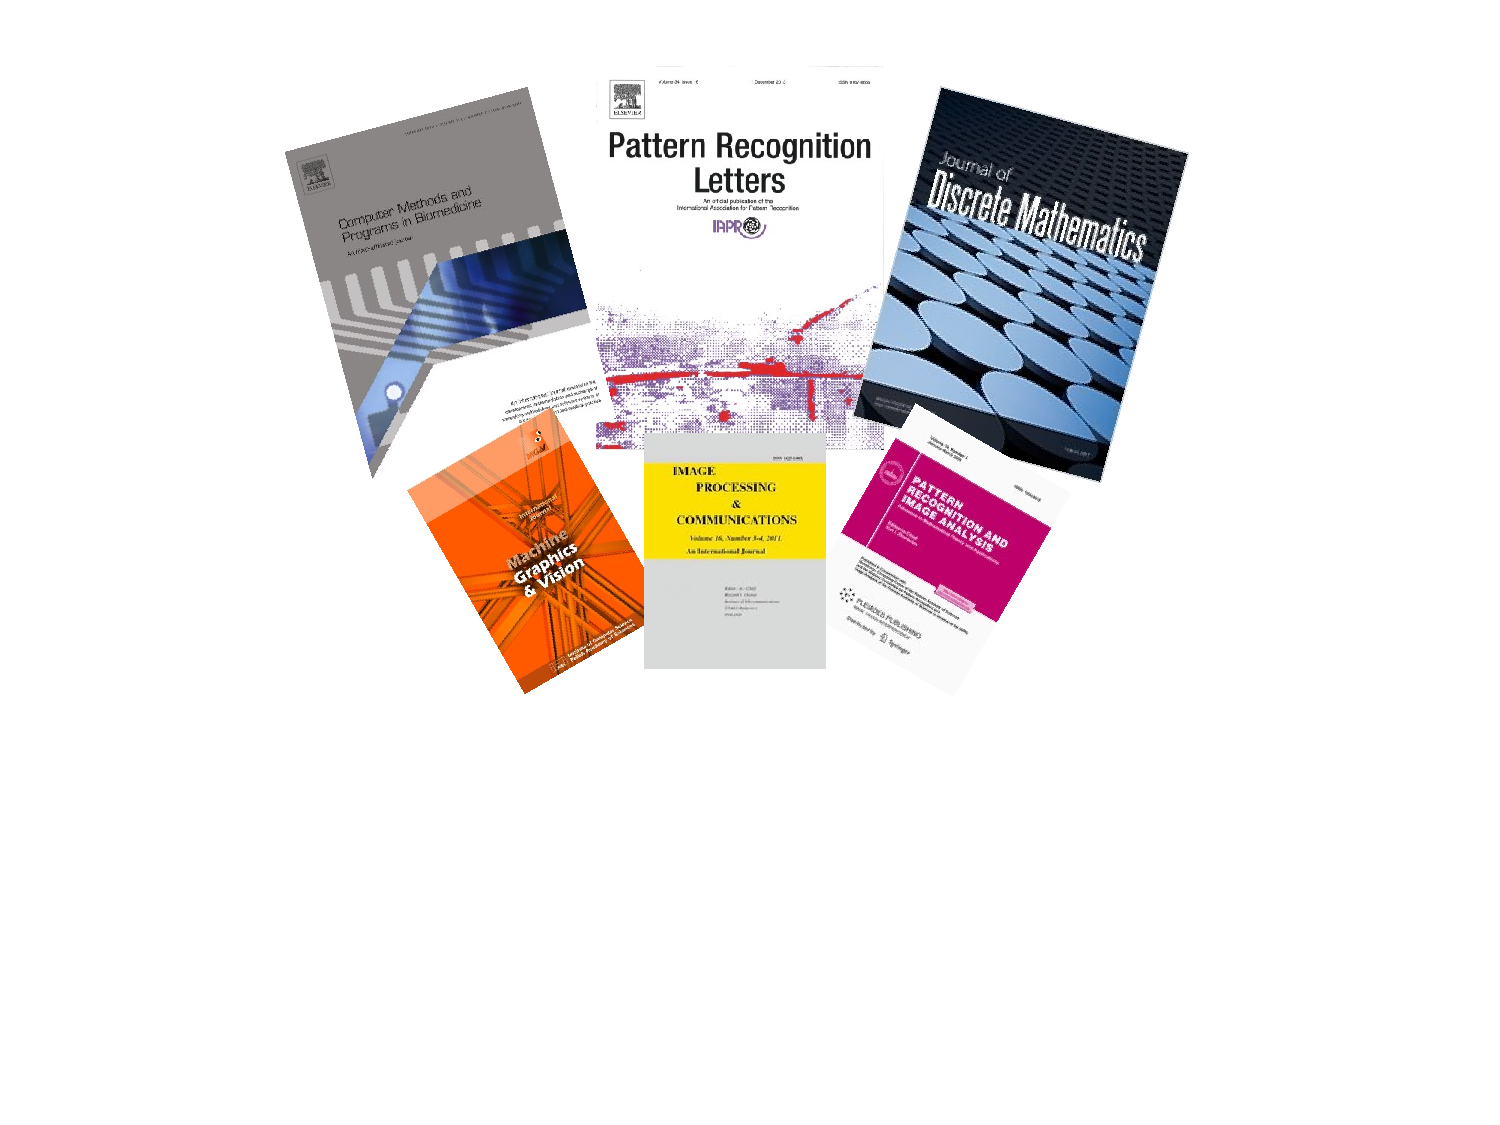
\includegraphics[angle=0, width=0.6\textwidth, viewport=110 200 630 510, clip]{./figures/tidsskrifter_AR_2013.pdf}
\caption{Journals with CBA staff in the editorial board.
\label{fig:journals_edit_CBA}}
\end{figure}
{\bf\noindent  Ewert Bengtsson}\\
\noindent International:
\begin{itemize}
%
%
\item
Senior lifetime member of the Institute of Electrical and Electronics Engineers (IEEE), 2004--\\
{\em Comment:} Member since 1974.Elevated to Lifetime Fellow as per 20150101.
%
\item
Member of the International Society for Optical Engineering (SPIE),
$\sim$2004--
%
\item
Member of the International Society for Analytical Cytology (ISAC),
2000--
%
\item
Associate Editor of {\em Computer Methods and Programs in Biomedicine,} 2012-2014\\
{\em Comment:} Published by Elsevier. Bengtsson was Editorial Board
member 1995-2011.
%
\item
Editorial Board member of {\em Machine Graphics \& Vision,} 1994--\\
{\em Comment:} Published by the Polish Academy of Sciences.
%
\item
Program Committee Bioimaging 2015, 12-15 January 2015, Lisbon, Portugal
% http://www.bioimaging.biostec.org/ProgramCommittee.aspx?y=2015
% The conference took place 2015 but all the work 2014, probably stays here as a comment until next year?
%
\item
Program Committee, 21st International Conference on Computer
Graphics, Visualization and Computer Vision (WSCG 2013), Plzen,
Czech Republic, June 2013.
%
\item
Management Committee, EU COST Action TD1201:
``Colour and Space in Cultural Heritage, COSCH'' 201305--\\
{\em Comment:} Bengtsson is responsible for coordinating the Swedish
participation.
%
\item
Finance chair ICPR2014, International Conference on Pattern Recognition, Stockholm, August 2014
% I do not know if it should be listed here since we are going to have a special ICPR section? 
%
\item
Expert evaluator for proposals to the Italian Ministry of Education, Industry and Research, Office V,  February-November 2014
\end{itemize}

%%%%%%%%%%%%%%%%%%%%%%%%%%%%%%%%%%%%
%%%%%%%%%%%%%%%%%%%%%%%%%%%%%%%%%%%%

\noindent National:
\begin{itemize}
\item
Member of the Royal Swedish Academy of Engineering Sciences (IVA), 2006--\\
{\em Comment:} Division VII: Basic and Interdisciplinary Engineering
Sciences.
%
\item
Member of the Royal Society of Sciences in Uppsala (Kungliga Vetenskaps-Societeten), 1998--\\
{\em  Comment:} Elected member of the oldest scientific society in
Sweden (founded 1710). %%
\item
Coordinating group of Medtech4Health, 201201-201406\\
{\em Comment:} Medtech4Health is a national Swedish initiative to
build a Strategic Innovation Area in medical engineering. And to apply for Vinnova Funding. 
The application was turned down in June 2014
%
\item
Board of Swedish Bioimaging, 201203-- \\
{\em Comment:} A Swedish network for researchers in biomedical
imaging and image analysis.
%
\item
Scientific board of Swedish Association for Medical Engineering and Physics, "Svensk förening för medicinsk teknik och fysik"  2013-- \\
% I can not find any official english name of this organisation so I have made a translation but suggest the Swedish name is included
%
\item
Program committee of Swedish Medical Engineering Days, "Medicinteknikdagarna", Gothenburgh, October 14-16, 2014. 
%
\item
Scientific board of Hillevi Fries Research Scholarship Foundation, 200611--\\
{\em Comment:} A Swedish foundation that accepts applications and
gives out research grants for urology research.
%
%
\item
Board of UpGIS, the network for Geographical Information Systems at
UU, 1999--
%
\item
UU Library Council member, 2011--
%
\item
IT strategy group at UU, 201206--201310\\
{\em Comment:} A committee headed by the university director to
create a new strategy for support of administrative IT at UU.
%
\item
Chair of Uppsala University committee to propose a new strategy for handling long term storage of scientific data.
201309--201403\\
%
\item
Chair of a joint committee by the Faculty of science and technology and the Faculty of medicine and pharmacy to develop a strategic plan for medical engineering research and education at Uppsala University. 201409--201501\\
%
\item
Representative of Uppsala University IT on the ICT committee of Uppsala Municipality, 2013--2014
%
\item
Expert advisor to the head of the Information Technology Unit of UU
administration, 2013--
%
\item
Board of the Dept. of Information Technology, UU, 201207--
%
\item
Head of Research (``forskningsprefekt") at the Dept. of Information
Technology, UU, 2013--
%
\item
Head of the research program ``Image analysis and man-machine
interaction," Dept. of Information Technology, UU, 1996-2014
\item
PhD education responsible professor for ``Computerized Image Processing", 1996-2014
\item
Licentiate Thesis, Matilda Landgren, Opponent, 20140131--20140131~
\item
Expert for evaluating chair in medical engineering for Link\"{o}ping University, 20141022--20141022~\\
{\em Comment:} Telephone conference deciding which of the 52 candidates were to be called to interview
\item
Expert evaluator of Dr Rodrigo Morenos application to become docent at Link\"{o}ping university . Finished April 16, 2014
%
% I have included a few new committees in my Squirrel input, I try not to repeat those here 
\end{itemize}



%%%%%%%%%%%%%%%%%%
%%    Gunilla   %%
% Uppdaterad 20150127 inkl squirrel
%%%%%%%%%%%%%%%%%%
{\bf\noindent Gunilla Borgefors}\\
\noindent International:
\begin{itemize}
\item
Fellow of the International Association for Pattern Recognition (IAPR), 1998--\\
{\em Comment:} 1st Vice President 1994-96, Secretary 1990-94, etc.,
etc.
%
\item
Fellow of the Institute of Electrical and Electronics Engineers, Inc. (IEEE), 2007--\\
{\em Comment:} Member since 1997. Senior member 1998.
%
\item
Editor-in-Chief of {\em Pattern Recognition Letters,} 2011--\\
{\em Comment:} Published by Elsevier. PRL is an official journal of
the International Association of Pattern Recognition. Borgefors was
Associate Editor/Area Editor 2004-2010.
%
\item
Editorial Board member of {\em Image Processing and Communications,} 1994--\\
{\em Comment:} Published by the Institute of Telecommunications,
Bydgoszcz, Poland.
%
\item
Editorial Board member of {\em Pattern Recognition and Image
Analysis: Advances in Mathematical Theory and Applications,} 1993--\\
{\em Comment: }Published by Interperiodica Publishing in cooperation
with the Russian Academy of Sciences.
%
\item
Editorial Board of the book series Computational Imaging and Vision,
2003-- \\
{\em Comment: } Published by Springer.
%
\item
Steering committee for Discrete Geometry for Computer Imagery (DGCI)
conferences, 2000--
%
\item
Steering committee for International Symposium on Mathematical
Morphology (ISMM), 2011--
\item
Dissertation committee of Darryl McClymont, School of Information Technology and Electrical Engineering, University of Queensland, Brisbane, Australia, 20140901--20141016~\\
{\em Comment:} Title: Computer assisted detection and characterisation of breast cancer in MRI~

\end{itemize}
%\newpage
%%%%%%%%%%%%%%%%%%%%%%%%%%%%%%%%%%%%%%%%
%%%%%%%%%%%%%%%%%%%%%%%%%%%%%%%%%%%%%%%%
\noindent National:
\begin{itemize}
\item
Member of the Royal Swedish Academy of Engineering Sciences (IVA), 2011--\\
{\em Comment:} Division VII: Basic and Interdisciplinary Engineering Sciences. %
%
\item
Member No. 19 of the Royal Society of Sciences in Uppsala (Kungliga Vetenskaps--Societeten), 2000--\\
{\em  Comment:} Elected member of the oldest scientific society in
Sweden (founded 1710).
%
\item
Member of Swedish Parliamentarians and Scientists, 1987--\\
{\em Comment:} Members are elected. Only one scientist per field
admitted.
%
\item
Board/Steering Committee for Onsala Space Observatory, 2011--
%
\item
Chair of the Celsius-Linn\'{e} committee, TN-faculty, UU, 201306--
\\
{\em Comment:} The committee selects the speakers for the annual
Celsius and Linn\'{e} lectures and organizes the following one-day
Symposium. Member since 2007.
%
\item
Advisory Board for CBA 2012-2014
\\{\em Comment:} One of two representatives for SLU.
%
\item
Expert evaluator for the application of Andrew Mehnert to become associate professor (docent) at Chalmers, G\"{o}teborg, 20140401--20140512
\item
Expert evaluator for an Associate Professor (lektor) in  Image reproduction at Dept.~of Science and Technology, Link\"{o}ping University, Campus Norrk\"{o}ping, 20140601--20140707
\item
Dissertation committee of Patrik Boberg, Lule\aa  Technical University, Lule\aa , 20140612~\\
{\em Comment:} Title: Imaging and Analysis Methods for Automated Weld Inspection
\item
Dissertation committee of Jimmy Azar, Dept.~of Information Technology, UU, 20141020~\\
{\em Comment:} Title: Automated Tissue Image Analysis Using Pattern Recognition
\end{itemize}


%%%%%%%%%%%%%%%%%%
%%    Anders Brun    %% .
%% Uppdaterad 2015-01-27
%%%%%%%%%%%%%%%%%%
National:
\begin{itemize}
\item
Board member, SSBA, 2014-- \\
{\em Comment:} Elected at SSBA yearly meeting
\end{itemize}
%%%%%%%%%%%%%%%%%%
%%    Ingrid    %% .
%% Uppdaterad 2015-02-02
%%%%%%%%%%%%%%%%%%
%\newpage
{\bf\noindent Ingrid Carlbom}\\
\noindent International:
\begin{itemize}
\item
Member of the Institute of Electrical and Electronics Engineers (IEEE), 1987--
%
\item
Member of Association for Computing Machinery (ACM), 1971--
%
\item
Member of ACM Special Interest Group on Computer Graphics and
Interactive Techniques (SIGGRAPH), 1976--
\item
Member of SIGMA XI, The Scientific Research Society $\sim$1979--
\item
Programme committee member, IEEE International Symposium on Biomedical Imaging (ISBI), 2014, 20140429--20140502
\item
Session organizer: "Advances in Computer-Aided Histopathology" at IEEE International Symposium on Biomedical Imaging (ISBI'14) held in Beijing, China, 20140428-20140502\\
\end{itemize}
%%


%%%%%%%%%%%%%%%%%%
%%    Anders Hast    %% .
%% Uppdaterad 2015-01-27
%%%%%%%%%%%%%%%%%%
{\bf\noindent Anders Hast}\\
%\noindent International:
%\begin{itemize}
%
%\end{itemize}
\noindent National:
\begin{itemize}
\item
Dissertation Committee Member, Andreas K\aa rsn\"{a}s, 20140412\\
{\em Comment:} PhD Thesis title: "mage Analysis Methods and Tools for Digital Histopathology Applications Relevant to Breast Cancer Diagnosis"
\end{itemize}


%%%%%%%%%%%%%%%
%%%%%%%%%%%%%%%
National:
\begin{itemize}
\item
Dissertation Committee of Erik Sintorn, Dept. of Computer Science and Engineering, Chalmers University of Technology, G\"{o}teborg, 20130226 \\
{\em Comment:} Title: Efficient real-time visibility testing
\end{itemize}



%%%%%%%%%%%%%%%%%%
%%   Christer Kiselman      %%
% Updated 2015-01-27
%%%%%%%%%%%%%%%%%%
{\bf\noindent Christer Kiselman}\\
\noindent International:
\begin{itemize}
\item
Program Committe for Discrete Geometry for Computer Imagery (DGCI 2014), 20140101--20140912
\item
Reference Group of the International Science Programme, 20140811\\
{\em Comment:} Meeting in Seoul, South Korea
\item
Evaluation of research at LIRIS, Lyon, 20140901--20150108~\\
{\em Comment:} LIRIS is the acronym of Laboratoire d'InfoRmatique en Image et Syst\`{e}mes d'information. Appointed by l'Agence d'\'{e}valuation de la recherche et de l'enseignement sup\'{e}rieur (AERES) (from 20141114  Haut Conseil d'\'{e}valuation de la recherche et de l'enseigment sup\'{e}rieur (HCERES)).

\end{itemize}
%%%%%%%%%%%%%%%%%%%%%%%%%%%%
%%%%%%%%%%%%%%%%%%%%%%%%%%%%
\noindent National:
\begin{itemize}
\item
Dissertation Committee of Vladimir Curic, Dept.~of Information Technology, UU, 20140523\\
{\em Comment:} Thesis title: Distance Functions and Their Use in Adaptive Mathematical Morphology
\end{itemize}
%%%%%%%%%%%%%%%%%%%%%%%%%%%%
%%%%%%%%%%%%%%%%%%%%%%%%%%%%



%%%%%%%%%%%%%%%%%%
%%    Cris      %%
% Updated 2015-01-27
%%%%%%%%%%%%%%%%%%
{\bf\noindent Cris Luengo}\\
\noindent International:
\begin{itemize}
\item
Senior member of the Institute of Electrical and Electronics Engineers (IEEE) 2010--\\
{\em Comment:} Member since 2001.
\item
Member of the International Society for Analytical Cytology (ISAC),
2006--
%
\item
Area Editor for Pattern Recognition Letters 2013-01--\\
{\em Comment:} Published by Elsevier. PRL is an official journal of
the International Association of Pattern Recognition. Luengo was
Associate Editor 2011-06--2012-12.
%
\item
Steering Committee, International Symposium on Mathematical Morphology, 2013--.
%
\item
Organizing Committee; Workshops, Tutorials and Contests Co-Chair; and Programme committee,
22nd International Conference on Pattern Recognition, Stockholm, 2014-08-24--28.
%
\item
Programme Committee, 22nd International Conference on Intelligent
Systems for Molecular Biology, Boston, MA, 2014-07-11--15.
\item
Programme Committee 22nd Int. Conf. on Pattern Recognition, 20140824--20140828
\end{itemize}
%%%%%%%%%%%%%%%%%%%%%%%%%%%%
%%%%%%%%%%%%%%%%%%%%%%%%%%%%
\noindent National:
\begin{itemize}
%
\item
Advisory Board for CBA 2012--
\\{\em Comment:} One of two representatives for SLU.
%
\item
Search Committee for a junior faculty member in Machine Learning for the Department of Information Technology, UU, 2014--2015
%
\item
Oponent for licentiate defence of Tobias Pahlberg, Division of Wood Science and Engineering, Lule\r{a} University of Technology, Skellefte\r{a}, 2014-02-14\\
{\em Comment:} Title: Wood Fingerprints: Recognition of Sawn Wood Products.
Supervisor: Olle Hagman.
%
\item
Dissertation committee of Janne West, Division of Radiological Sciences, Link\"{o}ping University, 2014-02-14\\
{\em Comment:} Title: Quantitative Magnetic Resonance Imaging of the Brain: Applications for Tissue Segmentation and Multiple Sclerosis.
Supervisor: \"{O}rjan Smedby.
%
\item
Dissertation committee of Richard Nordenskj\"{o}ld, Dept. of Radiology, Oncology and Radiation Science, UU, 2014-06-10\\
{\em Comment:} Title: Analysis of Human Brain MRI: Contributions to Regional Volume Studies.
Supervisor: Joel Kullberg.
\item
PhD Evaluation Committee,  Susanne Bornel\"{o}v, 20141003~\\
{\em Comment:} Supervisor: Jan Komorowski ~\\
Title: Rule-based models of transcriptional regulation and complex diseases ~\\
Dept. Cell and Molecular Biology, Computational and Systems Biology, Uppsala University~\\
%
\item
PhD Evaluation Committee,  Scott Holcombe, 20141216~\\
{\em Comment:} Supervisor: Staffan Jacobsson Sv\"{a}rd ~\\
Title: Gamma spectroscopy and gamma emission tomography for fuel performance characterization of irradiated nuclear fuel assemblies ~\\
Dept. of Physics and Astronomy, Applied Nuclear Physics, Uppsala University~\\
\end{itemize}
%%%%%%%%%%%%%%%%%%%%%%%%%%%%
%%%%%%%%%%%%%%%%%%%%%%%%%%%%


%%%%%%%%%%%%%%%%%%%
%%    Kristina    %%
% Uppdaterad 2015-01-27
%%%%%%%%%%%%%%%%%%%
%\newpage
{\bf\noindent Kristina Lidayova}\\
\noindent International:
\begin{itemize}
\item
Programme committee member, 1st International Conference on Bioimaging, BIOIMAGING 2014,Eseo, Angers, Loire Valley, France, 20140303--20140306
\end{itemize}

%%%%%%%%%%%%%%%%%%%
%%     Ingela    %%
% Uppdaterad 2015-02-04 by Ingela 
%% Added two entries from squirrel 2015-01-27
%%%%%%%%%%%%%%%%%%%
%\newpage
{\bf\noindent Ingela Nystr\"{o}m}\\
\noindent International:
\begin{itemize}
\item
President of the Executive Committee of International Association for Pattern Recognition (IAPR) 2014--\\
{\em Comment:} 2nd Vice President 2008--2010, Secretary 2010--2014 
%
\item
Local Arrangements Chair of the 22nd International Conference on Pattern Recognition (ICPR 2014), Stockholm, Sweden, August 2014 
%
\item
Program Committee Member of the 10th IEEE International Conference on e-Science, S�o Paulo, Brazil, October 2014 
\end{itemize}

%%%%%%%%%%%%%%%%%%%%%%%%%%%%
%%%%%%%%%%%%%%%%%%%%%%%%%%%%
\noindent National:
\begin{itemize}
\item
Member of the Royal Society of Arts and Sciences of Uppsala
(Kungliga Vetenskapssamh\"{a}llet i Uppsala), 2012--
%
\item
Member of the Board of the Faculty of Science and Technology, UU, 2011--2014 
%
\item
Member of the Docent committee of the Faculty of Science and Technology, UU,
2011--2014 
%
\item
Chair of the Advisory Board for the Centre for Image Analysis 2012--
\\{\em Comment:} One of two representatives for UU.
% 
\item
Member of the Council for Research Infrastructure (RFI), Vetenskapsr�det�, 2014-- 
%
\item
Evaluation Panel for grant applications to the Swedish Research
Council: Infrastructures for e-Science (``Beredningsgrupp 4''),
2011---
%
\item
Expert evaluator for the application of Claes Lundstr\"{o}m to become Associate Professor (Docent) at Link\"{o}ping University, 20140301--20140407
%
\item
Dissertation committee of Khoa Tan Nguyen, Dept. of Science and Technology, Link\"{o}ping University, Norrk\"{o}ping, 20140307~\\
{\em Comment:} Title: Supporting Quantitative Visual Analysis in Medicine and Biology in the Presence of Data Uncertainty
\end{itemize}



%%%%%%%%%%%%%%%%%%
%%    Alexandra    %% .
% Uppdaterad 2015-01-27
%%%%%%%%%%%%%%%%%%
{\bf\noindent Alexandra Pacureanu}\\
\noindent International:
\begin{itemize}
\item
Programme committee member, IEEE International Symposium on Biomedical Imaging (ISBI), 2014, 20140429--20140502~

\end{itemize}


%%%%%%%%%%%%%%%%%%
%%    Stefan    %% .
%%%%%%%%%%%%%%%%%%
{\bf\noindent Stefan Seipel}\\
%
\noindent International:
\begin{itemize}
\item
Program Committee, 21st International Conference on Computer
Graphics, Visualization and Computer Vision (WSCG 2013), Plzen,
Czech Republic, June 2013.
%
\item
Program committee, 17th International Conference on Information
Visualisation (iV 2013), London, U.K., July 2013.

\end{itemize}
%%%%%%%%%%%%%%%%%%%%%%%%%%%%%%%%
%%%%%%%%%%%%%%%%%%%%%%%%%%%%%%%%

\noindent National:
\begin{itemize}
\item
Chair of the Swedish Computer Graphics Association (SIGRAD),
201206--
%
\item
Expert evaluator for the Swedish Higher Education Authority
(``Universitetskanslers\"{a}mbetet"), subject IT\& New Media,
201209--201306.
%
\item
Scientific program committee, SIGRAD 2013, Norrk\"{o}ping, July
2013.
%
\item
Dissertation committee of Quan Ho, Norrk\"{o}ping, Dept. of Science
and Technology, Link\"{o}ping University, Campus Norrk\"{o}ping,
20130529\\
{\em Comment:} Title: Architecture and Applications of a Geovisual
Analytics Framework
%
\item
Dissertation committee of Patrik Lundblad, Dept. of Science and
Technology,
Link\"{o}ping University, Campus Norrk\"{o}ping, 20130530\\
{\em Comment:} Title: Applied Geovisual Analytics and Storytelling


\end{itemize}


%%%%%%%%%%%%%%%%%%%%
%% Ida-Maria
% Uppdaterad 2013
%%%%%%%%%%%%%%%%%%%
{\bf\noindent Ida-Maria Sintorn}\\
\noindent International:
\begin{itemize}
\item
Programme committee, 18th Iberoamerican Congress on Pattern
Recognition (CIARP 2013), Havanna, Cuba, Nov. 2013.
%
\item
Dissertation examiner of Swamidoss Isaac Niwas, Dept. of Electronics
and Communication Engineering, National Institute of Technology,
Tiruchirappalli, India, 201306 \\
{\em Comment:} Title: Complex Wavelet based Multiresolution Texture
Analysis of Microscopic Images for Breast Cancer Diagnosis.


\end{itemize}
%
\noindent National:
\begin{itemize}
\item
Treasurer of Swedish Society for Automated Image Analysis (SSBA), 2009-- \\
{\em Comment:} Board member 2008--.
\end{itemize}


%%%%%%%%%%%%%%%%%%
%%    Natasa     %% .
% Uppdaterad 2015-01-27
%%%%%%%%%%%%%%%%%%
{\bf\noindent Natasa Sladoje}\\
%\noindent International:
%\begin{itemize}
%%%%%
%\end{itemize}
\noindent National:
\begin{itemize}
\item
Dissertation Committee of Lennart Svensson, Swedish University of Agricultural Sciences, 20141124~\\
{\em Comment:} Title: Image Analysis and Interactive Visualization Techniques for Electron Microscopy Tomograms
\item
Dissertation Committee of Anders Landstr\"{o}m, Lule\aa   University of Technology, 20141125~\\
{\em Comment:} Title: Elliptical Adaptive Structuring Elements for Mathematical Morphology
%%%%
\end{itemize}


%%%%%%%%%%%%%%%%%%
%%    Robin     %% .
% Uppdaterad 2013
%%%%%%%%%%%%%%%%%%
{\bf\noindent Robin Strand}\\
\noindent International:
\begin{itemize}
%%%%
\item
Editorial Board member of {\em Journal of Discrete Mathematics,}
2013-- \\
{\em Comment:} Open access. Published by Hindawi Publishing
Corporation.
%
\item Chair of local organization and Programme committee member, 11th International Symposium on Mathematical Morphology (ISMM 2013), Uppsala, Sweden, May 2013.
%
\item
International advisory committee, International Conference on Signal
Processing, Image Processing and Pattern recognition (ICSIPR13),
Karunya Nagar Coimbatore, Tamil Nadu, India, Feb. 2013.
%
\item
Programme committee, 17th International Conference on Discrete
Geometry for Computer Imagery (DGCI 2013), Sevilla, Spain, Mar.
2013.
%
\item
Programme committee, 9th Workshop on Graph-based Representations in
Pattern Recognition (GbR2013), Vienna, Austria, May 2013.
%
\item
Programme committee, 18th Iberoamerican Congress on Pattern
Recognition (CIARP 2013), Havanna, Cuba, Nov. 2013.
%
\end{itemize}
%%%%%%%%%%%%%%%%%%%%%%%%%%%%%%%%%%%%%%%%%%
%%%%%%%%%%%%%%%%%%%%%%%%%%%%%%%%%%%%%%%%%%
\noindent National:
\begin{itemize}
\item
Member of the Electorial Board (``elektorsf\"{o}rsamlingen") of the
Faculty of Science and Technology, UU, 2011-2013
\end{itemize}

%%%%%%%%%%%%%%%%%%
%%    Carolina     %% .
% Updaterad 2015-01-27
%%%%%%%%%%%%%%%%%%
{\bf\noindent Carolina W\"{a}hlby}\\
\noindent International:
\begin{itemize}
\item
Dissertation committee of Barathy Mayurathan, Department of Statistics and Computer Science, Faculty of Science, University of Peradeniya, Sri Lanka , 20141104~\\
{\em Comment:} Title: Super resolution optical imaging -- image analysis, multicolor development and biological applications
\item
Programme committee member, IEEE International Symposium on Biomedical Imaging (ISBI), 2014, 20140429--20140502~
%
\end{itemize}
%%%%%%%%%%%%%%%%%%%%%%%%%%%%
%%%%%%%%%%%%%%%%%%%%%%%%%%%%
\noindent National:
\begin{itemize}
\item
Dissertation committee of Daniel R\"{o}nnlund, Dept. of Experimental Biomolecular Physics, KTH, 20140228~\\
{\em Comment:} Title: Efficient and Compact Codebook Design for Scene Analysis and Object Localisation
%
\item
Dissertation committee of Arash Sanamrad, Dept. of Cell and Molecular Biology, UU, 20140905~\\
{\em Comment:} Title: Biological Insights from Single-Particle Tracking in Living Cells
\item
Member of the Electorial Board (``elektorsf\"{o}rsamlingen") of the
Faculty of Science and Technology, UU, 2014-2016
\end{itemize}
%\end{document}
